% CREATED BY DAVI FRISK, 2015
\chapter{Results}
section{Manual Analysis}
For conflicts in the category SameSignatureCM, we found that if one version have the same code as the other version but with some additional code, that version was often chosen. Superset and Recent were each chosen for more than half of the cases, as can be seen in Table (no).

\begin{table}
\begin{tabular}{ p{8cm} p{6cm} }
\hline
\multicolumn{1}{c}{\textbf{Category}} & \multicolumn{1}{c}{\textbf{Number of cases out of 26}}\\
Superset & 18 (~69\%)\\
Recent & 15 (~58\%)\\
Subset & 4 (~15\%)\\
\end{tabular}
\caption{Resolution categories statistics in the manual analysis}\label{table:rcsitma}
\end{table}

For some of the cases that were chosen as resolution, one or more if-statements had been introduced in the version that was chosen which the other version didn’t have. We also saw that one of the cases chose a version with more error handling than the version that wasn’t chosen.

section{Automatic Analysis}
The automatic analysis that was conducted on the 20 top starred Java projects on GitHub yielded, after our filtering, 1958 conflicts.

subsection{Selected Version}
One of the results is that in more than 75\% of the studied cases, the left version was chosen, that is, the version in the commit that was checked out at the time of merging.

  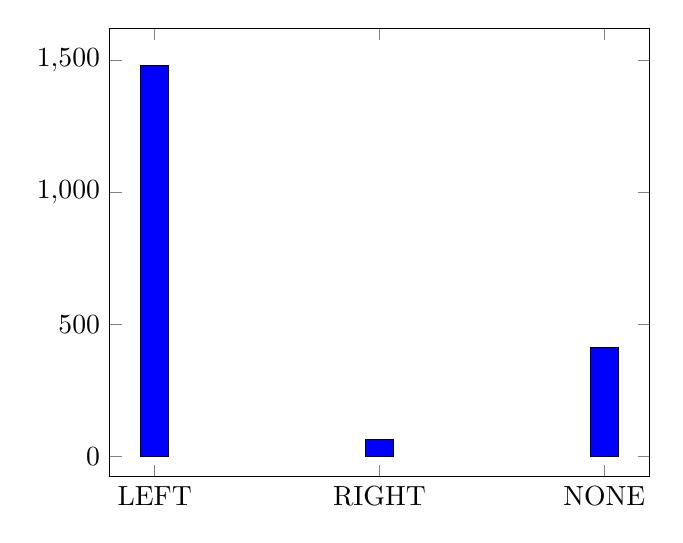
\begin{tikzpicture}
       \begin{axis}[
           symbolic x coords={LEFT, RIGHT, NONE},
           xtick=data
         ]
           \addplot[ybar,fill=blue] coordinates {
               (LEFT,   1481)
               (RIGHT,  65)
               (NONE,   412)
           };
       \end{axis}
   \end{tikzpicture}

\subsection{Keywords}
Another result is that for conflicts, where one of the versions contains more instances of the keyword if than the other, the version with the higher frequency is chosen in 84\% of the cases. However, for the print-, log- and try keywords, the results show that it is less common to choose the version which contain more of those keywords. Table(no) lists the total number of cases where the frequency of occurrence of the keyword differs.
\begin{table}
\begin{tabular}{ p{8cm} p{6cm} }
\hline
\multicolumn{1}{c}{\textbf{Keyword}} & \multicolumn{1}{c}{\textbf{Total number of cases}}\\
if & 616\\
print & 21\\
log & 16\\
try & 35\\
\end{tabular}
\caption{Keywords}\label{table:keywords}
\end{table}


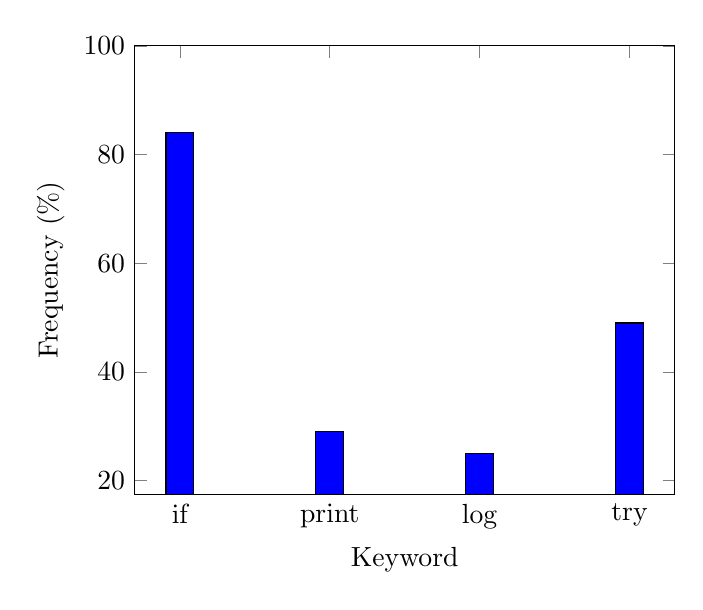
\begin{tikzpicture}
      \begin{axis}[
          symbolic x coords={if, print, log, try},
          xtick=data,
          ymax=100,
          ylabel={Frequency (\%)},
          xlabel={Keyword}
        ]
          \addplot[ybar,fill=blue] coordinates {
              (if, 84)
              (print, 29)
              (log, 25)
              (try, 49)
          };
      \end{axis}
  \end{tikzpicture}


